\documentclass[12pt,twoside]{article}

%\usepackage{amsthm}%
\usepackage{amsmath}
\usepackage{amssymb}
\usepackage{amsfonts}
\usepackage[margin=1in]{geometry}
\usepackage{enumerate}
\usepackage{verbatim}
\usepackage{graphicx}
\usepackage{hyperref}
\usepackage[]{algorithm2e}

\newenvironment{proof}{\noindent{\bf Proof:} \hspace*{1mm}}{
	\hspace*{\fill} $\Box$ }
\newenvironment{proof_of}[1]{\noindent {\bf Proof of #1:}
	\hspace*{1mm}}{\hspace*{\fill} $\Box$ }
\newenvironment{proof_claim}{\begin{quotation} \noindent}{
	\hspace*{\fill} $\diamond$ \end{quotation}}

\newtheorem{thm}{Theorem}
\newtheorem{lemma}[thm]{Lemma}

\newcommand{\mbf}{\mathbf}
\newcommand{\mrm}{\mathrm}

\newenvironment{centered}[0]{%
  \begin{list}{}{%
    \setlength{\topsep}{0pt}%
    \setlength{\leftmargin}{.25in}%
    \setlength{\rightmargin}{.25in}%
    \setlength{\listparindent}{\parindent}%
    \setlength{\itemindent}{\parindent}%
    \setlength{\parsep}{\parskip}%
  }
  \item[]}{\end{list}}
\newcommand\abs[1]{\left|#1\right|}
\newcommand\given[1][]{\:#1\vert\:}
\newcommand{\legendre}[2]{\genfrac{(}{)}{}{}{#1}{#2}}
\setcounter{tocdepth}{1}
\newtheorem{theorem}{Theorem}


\title{Constructing Pairing-Friendly Elliptic Curves }
\date{\today}
\author{ Peter Manohar, Xingyou Song} 

\begin{document}

\maketitle

\abstract{This report covers some of the fundamental aspects of elliptic curve construction. Specifically, we will focus on the Cocks-Pinch and Dupont-Enge-Morain methods for curve construction. We start by giving an overview of important concepts about elliptic curves needed for understanding these two methods, and then we will state and explain the two algorithms. Finally, we explore some of the applications of elliptic curves to cryptography. 
}

\tableofcontents

\section{Introduction}



\subsection{Elliptic Curves}

For our project, we shall define an elliptic curve to be a curve of the form:
\begin{equation}
E: \ y^2 = x^3 + Ax + B,
\end{equation}
where $A$ and $B$ are elements of some field $\mathbb F$, with char$(\mathbb F) \ne 2,3$. The curve $E$ is nonsingular if $\partial F / \partial x$ and $\partial F / \partial y$ are not simultaneously $0$ for all points on $E$. It follows that $E$ is nonsingular $\iff x^3+ Ax+ B$ has distinct roots. Through Vieta's formulas, $E$ has distinct roots $\iff ((r_{1} - r_{2})(r_{1} - r_{3})(r_{2} - r_{3}))^{2} = -(4A^{3} + 27B^{2})$ is nonzero. Therefore, we shall also require that the discriminant of $E$,
\begin{equation} 
\Delta = -16(4A^{3} + 27B^{2})
\end{equation}
is nonzero. 
The $j$-invariant of $E$ is defined by:
\begin{equation}
j(E) = 1728 \frac{4A^{3}}{4A^{3} + 27B^{2}} \, .
\end{equation}
\subsection{Group Law} 
The points on an elliptic curve form an additive abelian group. We shall define the group law geometrically. \\
Let $P = (x_p, y_p), Q = (x_q, y_q)$. A line through $P$ and $Q$ intersects $E$ at a third point, $R = (x_r,y_r)$. We define $P + Q := (x_r,-y_r)$. Pictorally, this looks like \\
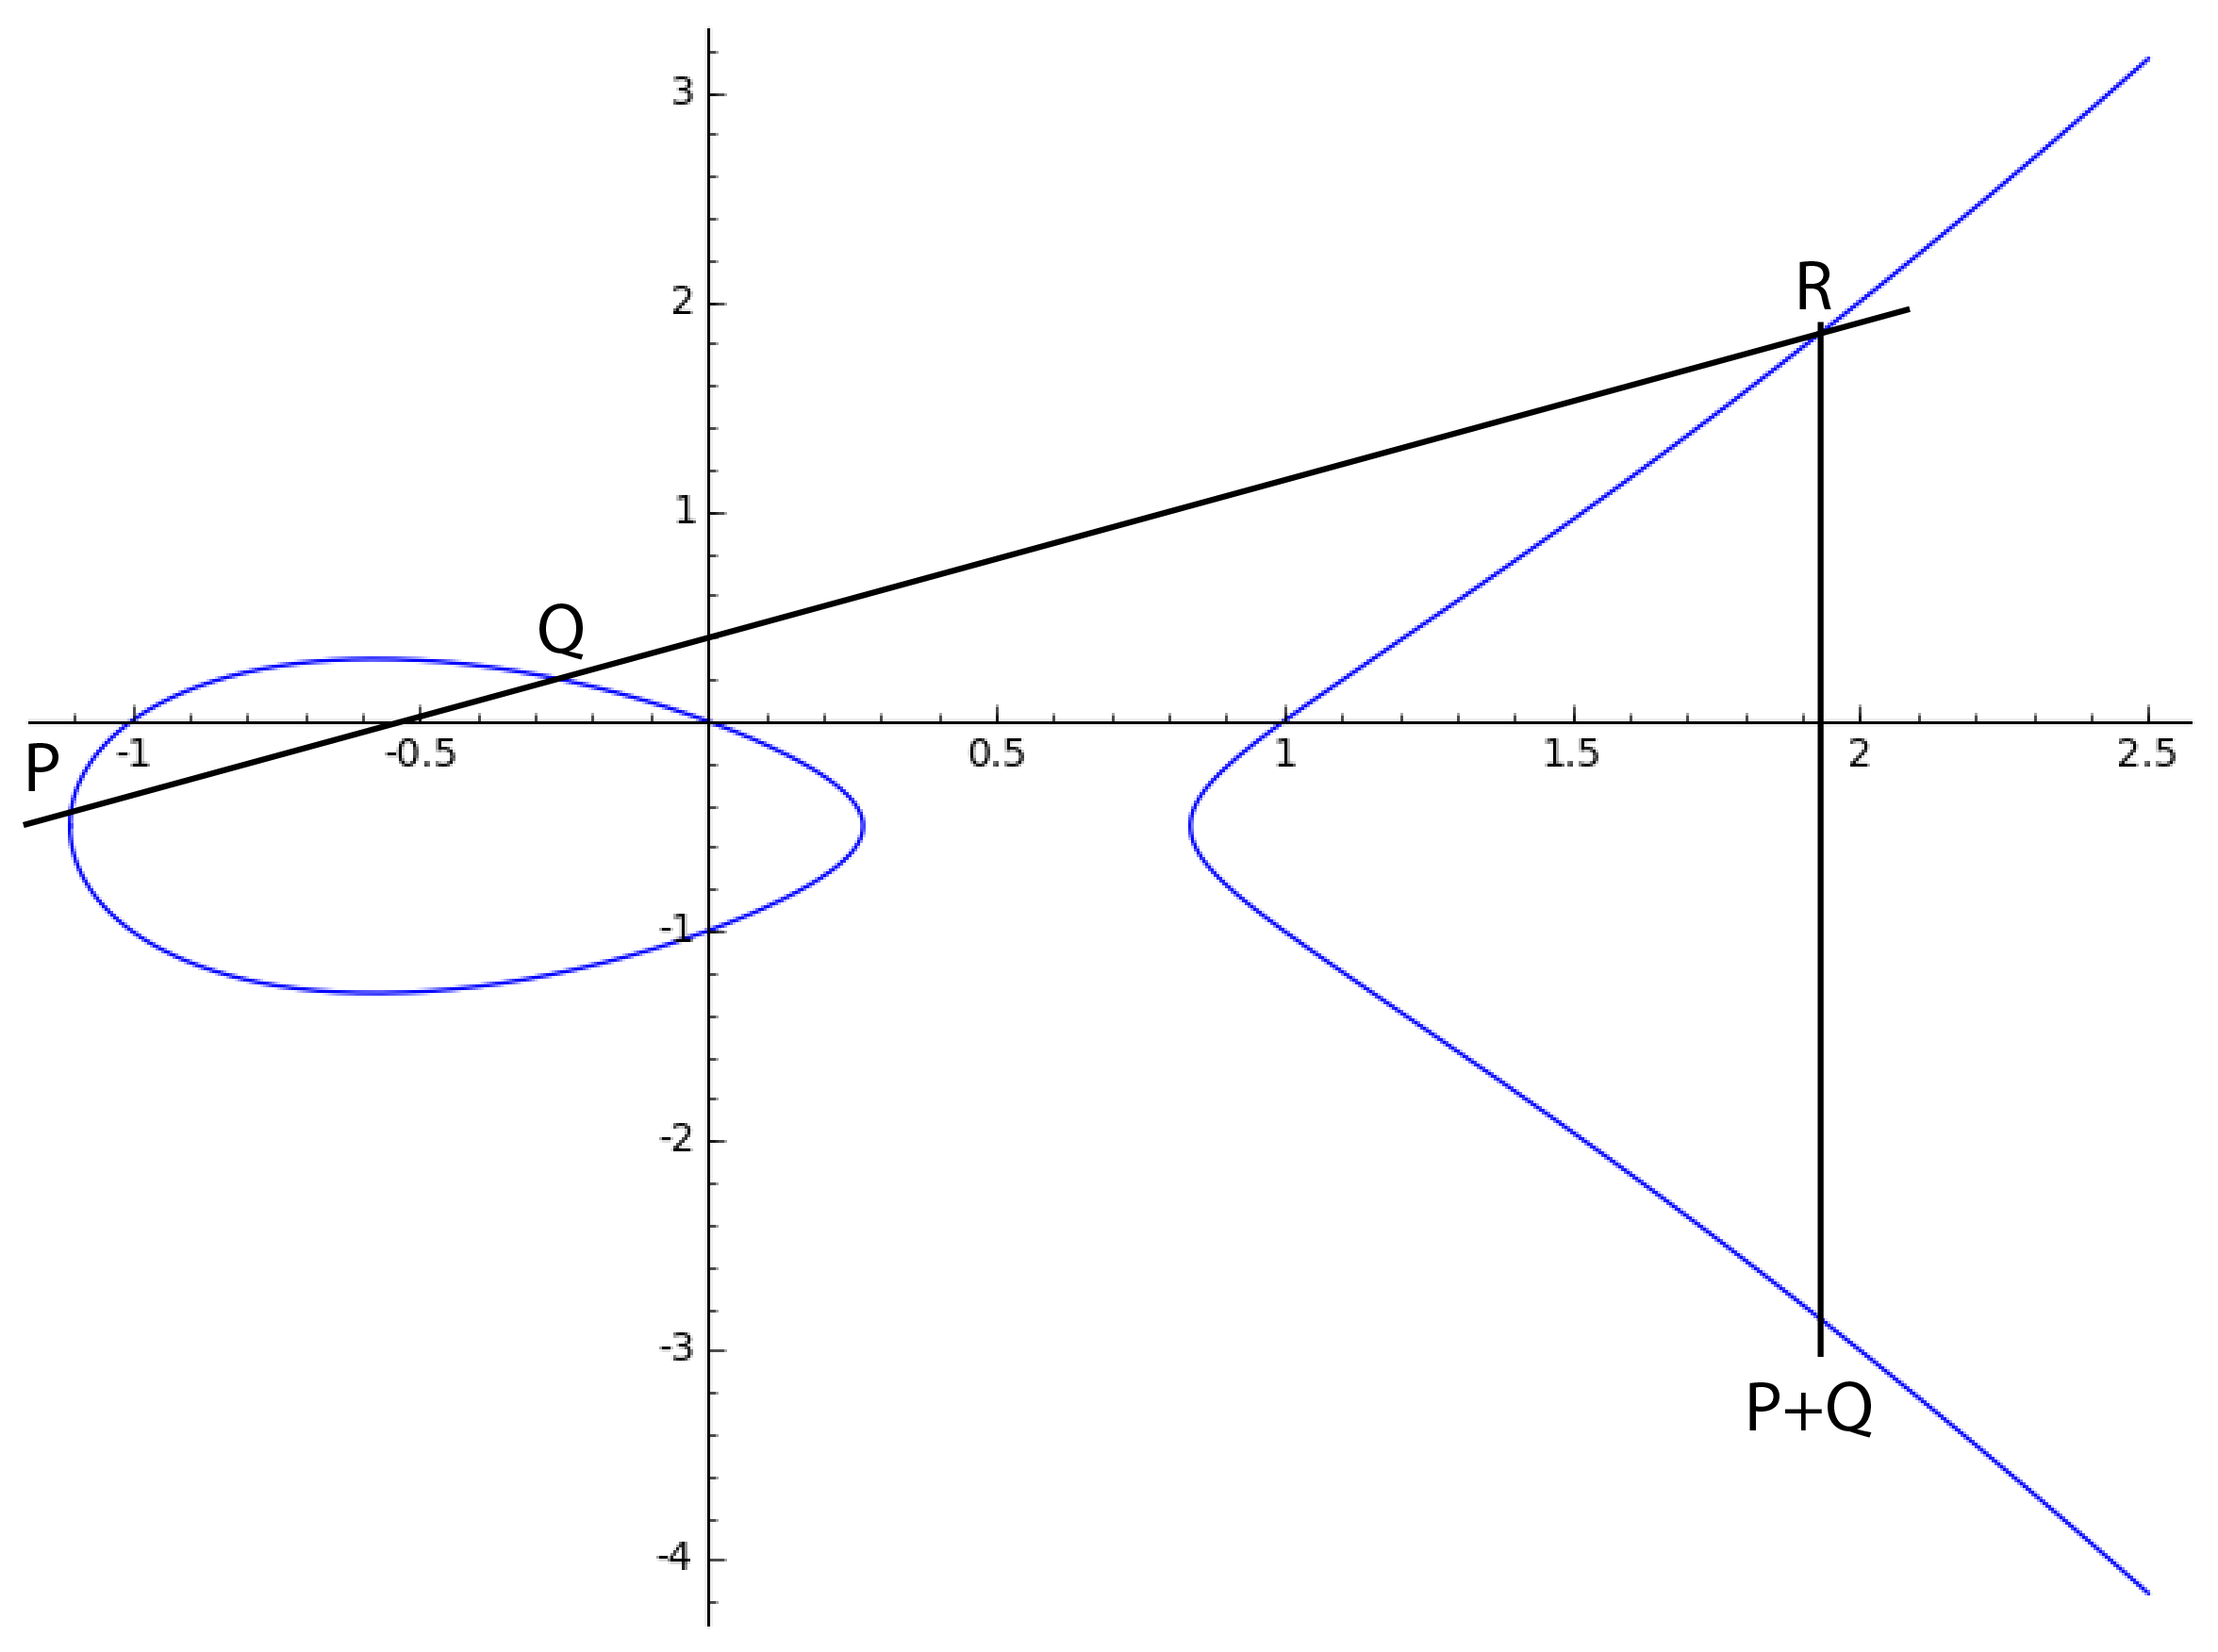
\includegraphics[width=6in]{grouplaw.png}
The group law can also be defined in terms of algebraic formulas, which can be found in [SIL08, III.2].

\subsection{Notation}
\begin{itemize}
\item $\mathbb F$ is a field
\item $\overline{\mathbb F}$ is the algebraic closure of $\mathbb F$
\item $\mathbb F_p$ is a field with $p$ elements, where $p$ is prime
\item $E(\mathbb F) = \{(x,y) \in \mathbb F \times \mathbb F \given E(x,y) = 0\}$
\item $\phi$ is an isogeny (or endomorphism)
\item $\phi_p$ is the Frobenius endomorphism
\item $[n]$ is the multiplication by $n$ map
\end{itemize}

\section{Background}

In this section, we shall define key concepts needed for our report. We will prove some of the more important results, and cite a source otherwise.

\subsection{Isogenies} 
An isogeny of two elliptic curves $E_1$ and $E_2$ defined over a field $\mathbb F$ is a nonconstant morphism $\phi: E_1 \to E_2$, where $\phi$ is a group homomorphism from $E_1(\overline{\mathbb F}) \to E_2(\overline{\mathbb F})$. $E_1$ and $E_2$ are isomorphic if there exist isogenies $\phi_1,\phi_2$ where $\phi_1: E_1 \to E_2$ and $\phi_2: E_2 \to E_1$ such that $\phi_2 \circ \phi_1 =  $ Identity.

\subsubsection{Separable and Inseparable Isogenies}
Any isogeny $\phi$ can be expressed as $\phi(x,y) = ({u(x)}/{v(x)}, y \, {s(x)}/{t(x)})$, where $u,v,s,t \in \mathbb F[x]$, and $\gcd(u,v) = \gcd(s,t) = 1$.
An isogeny is separable if $({u}/{v})' = 0$, and is inseparable otherwise. The degree of an isogeny is defined as $\deg(\phi) := \max(\deg(u), \deg(v))$.
For any separable isogeny $\phi$, $\deg(\phi) = \abs{ \ker \phi}$. [SUTH15]

\subsubsection{Dual isogenies}
\begin{theorem}
Let $\phi: E_1 \to E_2$ be an isogeny. Then $\exists$ a unique $\hat{\phi}: E_2 \to E_1$ such that $\hat \phi \circ \phi = [n]$, where $n = \deg(\phi)$.
\end{theorem}
\noindent The proof of this can be found in either [SIL08] or [SUTH15]. Furthermore, for any two isogenies $\phi_1$ and $\phi_2$, $\widehat{\phi_1 + \phi_2} = \hat \phi_1 + \hat \phi_2$.
\subsection{Endomorphisms}

An endomorphism is an isogeny from $E$ to itself. The endomorphisms of $E$ form a ring, where addition is addition of functions and multiplication is function composition.

\subsubsection{Examples}

The map $[n]: E \to E$, where $[n]P = P + P + \dots + P$ ($n$ times) is an endomorphism.
\\ \\
\noindent If $E$ is defined over $\mathbb F_p$, the Frobenius map $\phi_p: E \to E$ defined by $\phi_p(x,y) := (x^p, y^p)$ is an (inseparable) endomorphism.

\subsubsection{Trace of an Endomorphism}

\begin{theorem}
For any endomorphism $\phi$, $\phi + \hat \phi = 1 + \deg(\phi) - \deg(1-\phi)$, where we can regard the RHS as an endomorphism by the map $n \mapsto [n]$.
\end{theorem}
\begin{proof}
As endomorphisms, 
\begin{flalign*}
& [\deg(1-\phi)] = \widehat{(1-\phi)}(1-\phi) = (\hat 1 - \hat \phi)(1-\phi) = (1 - \hat \phi)(1-\phi) \\
&= 1 - \hat \phi - \phi + \hat \phi \circ \phi = 1 - \hat \phi - \phi + [\deg(\phi)] \\
& \implies \phi + \hat \phi = 1+ [\deg(\phi)] - [\deg(1- \phi)] 
\end{flalign*}
\end{proof}
\\
By the above theorem, we can now define trace$(\phi) := \phi + \hat \phi$.
\begin{theorem}
$\#E(\mathbb F_p) = p + 1 - t$, where $t = {\rm trace}(\phi_p)$
\end{theorem}
\begin{proof}
The fixed field of $\phi_p$ is $\mathbb F_p$, and $1- \phi_p$ is separable (see [SUTH15]). Therefore, $\ker(1- \phi_p) = \#E(\mathbb F_p)$. It is clear that $\deg(\phi_p) = p$ by definition ($u(x) = x^p$ and $v(x) = 1$). We have that
\begin{flalign*}
&\ker(1-\phi_p) = \deg(1-\phi_p) = 1 + \deg(\phi_p) - {\rm trace}(\phi_p) = p + 1 - t \\
&\implies \#E(\mathbb F_p) = p + 1 -t
\end{flalign*}
\end{proof}


\bigskip

\begin{comment}
\begin{theorem} 
If $K$ is a field of characteristic $0$ or does not divide $m$, then
$ E[m] \simeq Z_{m} \oplus Z_{m}$.  
\end{theorem} 
The proof of this is mainly using the fundamental theorem of abelian groups, and analyzing the decomposition of the torsion group (TODO?) 
\end{comment}


\subsection{$j$-invariant} 

\begin{theorem}
Two elliptic curves $E_1(\mathbb F)$ and $E_2(\mathbb F)$ are isomorphic over $\overline{\mathbb F} \iff j(E_1) = j(E_2)$. Furthermore, $\forall j_0 \in \overline{\mathbb F}$, $\exists$ an elliptic curve $E(\mathbb F)$ such that $j(E) = j_0$.
\end{theorem}
The proof requires some lengthy algebraic manipulation, which can be found in [SIL08, III.1]. As a consequence of the proof, for any $j \in \overline{\mathbb F}$, we can define a canonical elliptic curve $E$ associated with this $j$-invariant. We see that 

  
\begin{flalign} 
& E: y^{2}  = x^{3} + \frac{3j}{1728 - j}x + \frac{2j}{1728 - j} \text{\ if \ } j \ne 0, 1728\\
\nonumber & E: y^2 = x^3 + 1 \text{\ if \ }  j = 0 \\
\nonumber & E: y^2 = x^3 + x \text{\ if \ } j = 1728
\end{flalign}

\begin{comment}
A question arises when two elliptic curves over a field $E_{1}(K), E_{2}(K)$ are have a bijective isogeny, i.e. are isomorphic with respect to the group law. 
An intuitive answer is that the points on elliptic curves be transformed algebraically, which will use different Weierstrass Equations

Note the transformation  

\begin{align*}
x' = \mu^{2}x \\   
y' = \mu^{3}y 
\end{align*}

implies, after plugging into the Weierstrass equation,

\begin{equation} 
(y')^{2} = (x')^{3} + \mu^{4}Ax' +\mu^{6}B \implies (y')^{2} = (x')^{3} + A'x' + B'  
\end{equation} 
where $A' = \mu^{4}A, B' = \mu_{6}B$. $\mu$ may not exist in the field $K$, but only in its closure $\bar{K}$. 

From here, we define the j-invariant $j$ of a Weierstrass Form to be 
\begin{equation} 
j(E) = 1728 \frac{4A^{3}}{4A^{3} + 27B^{2}}
\end{equation}

Note that the $j$ invariant is homogenous; scalings of the form from (5) will still leave $j$ constant. Given a $j$, then the canonical elliptic curve associated with this j-invariant will be 


\subsubsection{Example}
$E_1(\mathbb F)$ and $E_2(\mathbb F)$ can be isomorphic over $\overline{\mathbb F}$, but not over $\mathbb F$. As an example, consider the curves $E_1: y^{2} = x^{3} - 25x$, $E_2: y^{2} = x^{3} - 4x$ have $j=1728$. $\#E_1(\mathbb Q) = \infty$ because we can just take an infinite group with generator $(-4,6)$ but $\#E_2(\mathbb Q) < \infty$ because the only points on it $\infty, (2,0), (-2,0), (0,0)$ form a finite abelian group. \\
The transformation $(x,y) \rightarrow (\mu^{2}x, \mu^{3}y)$, $\mu = \frac{\sqrt{10}}{2}$ establishes an isomorphism over $\mathbb Q(\sqrt{10})$, but no such isomorphism exists over $\mathbb Q$.

From this example, we can see that we do not necessarily need the full closure $\overline{\mathbb F}$; we only needed $d \in \mathbb F$ such that $d= \mu^{2}$, which in this case was $\mathbb Q(\sqrt{10})$, which gives rise to the idea of quadratic twists. 
\end{comment}
\subsection{Twists} 
Two curves $E_1(\mathbb F)$ and $E_2(\mathbb F)$ are {\it twists} if they are isomorphic over $\overline{\mathbb F}$ but not over $\mathbb F$.
\subsubsection{Quadratic Twists}
In particular, we are interested in quadratic twists. If $E: y^2 = x^3 + Ax+ B$ is an elliptic curve defined over $\mathbb F$, and $d \in \mathbb F$ is a nonsquare, then we define the {\it quadratic twist of E} as $\tilde E: y^2 = x^3 + d^2Ax + d^3B$.

\begin{theorem}
If $E: y^2 = x^3 + Ax + B$ is an elliptic curve over $\mathbb F_p$ with $\#E(\mathbb F_p) = p+ 1 - t$, then $\#\tilde E(\mathbb F_p) = p+ 1 + t$
\end{theorem}
\begin{proof}
Let $\legendre{\cdot}{p}$ be the legendre symbol mod $p$. For any $x \in \mathbb F_p$, we see that $1 + \legendre{x^3+Ax+B}{p} = $ \# of points on $E$ with $x$-coordinate $x$. Therefore, 
\begin{flalign*}
\#E(\mathbb F_p) = 1 + \sum_{x \in \mathbb F_p} {\left[ 1 + \legendre{x^3+Ax+B}{p} \right]} = p + 1 + \sum_{x \in \mathbb F_p} {\legendre{x^3+Ax+B}{p}}
\end{flalign*}
Since $\mathbb F_p$ is a field, $\forall x \in \mathbb F_p$, $\exists x' \in \mathbb F_p$ such that $d x' = x$. Therefore, for $\tilde E(\mathbb F_p)$, we have that
\begin{flalign*}
&\#\tilde E(\mathbb F_p) = 1 + \sum_{x \in \mathbb F_p} {\left[1 + \legendre{(dx)^3+A(dx)+B}{p}\right]} = p + 1 + \sum_{x \in \mathbb F_p} {\legendre{d^3(x^3+Ax+B)}{p}} \\
& = p + 1 + \sum_{x \in \mathbb F_p} {\legendre{d}{p} \legendre{d^2}{p} \legendre{x^3+Ax+B}{p}} = p + 1 - \sum_{x \in \mathbb F_p} {\legendre{x^3+Ax+B}{p}}
\end{flalign*}
\end{proof}
\subsection{Pairings and Pairing-Friendly Curves}
Let $G$ be an additive abelian group of order $p$, a prime, and let $G'$ be a multiplicative group of order $p$. A pairing is a bilinear map $e: G \times G \to G'$ satisfying:
\begin{enumerate}
\item (bilinearity) $e(P_1 + P_2, P_3) = e(P_1,P_3)e(P_2,P_3)$ and $e(P_1, P_2+P_3) = e(P_1,P_2)e(P_1,P_3)$ \\ $\forall P_1,P_2,P_3 \in G$
\item (non-degeneracy) $e(P,P) \ne 1$, where $G = \mathopen{<} P \mathopen{>}$
\item (computability) $e$ is efficiently computable
\end{enumerate} [PAIR91]
\subsubsection{Weil and Tate Pairings}
Let $E[r] = \{ P \in E(\mathbb F_p) \given rP = O\}$ be the $r$-torsion group of $E(\mathbb F_p)$.
\\ \\
\noindent The Weil Pairing is a map $e_r: E[r] \times E[r] \to \mu_r$, where $\mu_{r}$ is the set of $r$th roots of unity in $\overline{\mathbb F_p}$. \\ 

\noindent The Tate Pairing is a map: $\tau_r: E(F_p)[r] \times E(F_p)[r]/ rE(F_p) \to \mu_r$, where $\tau_r(P,Q) = e_r(P, R - \phi_p(R))$, where $R$ satisfies $r R = Q$. [WASH08]



 \subsubsection{Embedding Degree}
 
We do not need the full algebraic closure $\overline{\mathbb F_p}$ to determine $\mu_r$. Instead, we can find a positive integer $k$ such that $\mu_r \subset \mathbb F_{p^k}$, that is, we require only a finite degree algebraic extension. We define the embedding degree $k$ of $E(\mathbb F_p)$ with respect to $r$ as $k:= [\mathbb F_p(\mu_r) : \mathbb F_p]$, the degree of the extension field. Therefore, we can regard $k$ as the smallest positive integer such that $\mu_r \subset \mathbb F_{p^k}$.
\\ \\
\noindent Alternatively, suppose that $k$ is the smallest positive integer such that $\mu_r \subset \mathbb F_{p^k}$.  $\mu_r \subset \mathbb F_{p^k} \iff r \Big |  \# \mathbb F^*_{p^k}$ (since multiplicative groups of finite fields are cyclic) $ \iff p^k-1 \equiv 0 \mod r \iff p$ is a primitive $k$th root of unity mod $r$ (since we picked $k$ to be minimal). 
\\ \\
\noindent Therefore, the embedding degree $k$ is the smallest positive integer satisfying $p^k \equiv 1 \mod r$.

\subsubsection{Pairing-Friendly Curves}
The Weil/Tate Pairing is efficiently computable when $k$ is small, as computing the pairings requires computation in $\mathbb F_{p^k}$. A curve with efficiently computable pairings is {\it pairing-friendly}. Pairing-friendly curves are rare. In general, if $r \approx p$, then $\Pr[$pairing-friendly curve$] = O(\frac{\log^3 p}{p})$. [IM98]

\subsection{Ordinary Curves}

{\bf Definition: } $E(\mathbb F_p)$ is ordinary if $\#E[p] = p$. If $\#E[p] \ne p$ ($\#E[p] = 1$) then $E(\mathbb F_p)$ is supersingular. \\


\noindent For this project we are interested in constructing ordinary curves, as supersingular curves are vulnerable to attacks since they have embedding degree $2$ over $\mathbb F_p$ for $p \geq 5$. We will see that the curve generation algorithms we use only construct ordinary curves.

\subsection{Complex Multiplication}
\subsubsection{Complex Lattice}
\begin{theorem} 
Let $\omega_{1}, \omega_{2}$ be linearly independent points in $C$.  Define the lattice 
$$ L = Z\omega_{1} + Z \omega_{2}$$ Then there exists an elliptic curve that is isomorphic to $\mathbb{C}/ L$. 
\end{theorem}
{\bf Proof Sketch:} \\

\noindent The Weierstrass $\wp (z) $ function is: 

\begin{equation} 
\wp(z) = \frac{1}{z^{2}} + \sum_{\omega \in L}\left(\frac{1}{(z-\omega)^{2}} - \frac{1}{\omega^{2}}\right) \, .
\end{equation}  
$\wp(z)$ is convergent, doubly periodic with periods $\omega_1$ and $\omega_2$, and is holomorphic on $\mathbb C$ everywhere except on $L$. The derivative of $\wp(z)$ is 
\begin{equation} 
\wp ' (z) = -2 \sum_{\omega \in L} \frac{1}{(z- \omega)^{2}} \, .
\end{equation} 
$\wp(z)$ gives an isomorphism from $\mathbb{C}/L$ to $E(\mathbb{C})$, by the map $$z \rightarrow ( \wp(z), \wp' (z)), \> \> \> \> \> 0 \rightarrow O $$ with $E$ being defined as 
\begin{equation} 
E: y^{2} = 4x^{3} - g_{2}x - g_{3} 
\end{equation} 
where $g_{2} = 60G_{4}, g_{3} = 140G_{6}$, and $G_{k}(L) = \sum_{\omega \in L}\omega^{-k}$ is the Eisenstein series of weight $k$.

\noindent It can be shown that addition of points on $E(\mathbb C)$ corresponds to addition of points in $\mathbb C/L$. [SUTH15] Formally:

\begin{equation} 
\left( \wp(z_{1}), \wp'(z_{1}) \right) + \left( \wp(z_{2}), \wp'(z_{2}) \right) = \left( \wp(z_{1} + z_{2}), \wp'(z_{1} + z_{2}) \right) \, .
\end{equation} \\ \\
\noindent  We can also relate the $j$-invariant on curves to the $j$-function of a complex lattice. First, observe that we can rescale our lattice $L$ to $Z\tau + Z$ where $\tau = {w_{1}}/{w_{2}}$, while preserving $\mathbb C/L$ as a group. The $j$-invariant of $L$ is
\begin{equation}
j(\tau) = 1728 \frac{g_{2}^{3}}{g_{2}^{3} - 27 g_{3}^{2}} \, .
\end{equation} 

 
\noindent The theorem states that every lattice $\mathbb C/L \cong E(\mathbb C)$ for some elliptic curve $E$. However, it turns out that the converse is also true. Namely, $E(\mathbb C) \cong \mathbb C/L$ for some lattice $L$. This establishes an isomorphism between the endomorphism rings of $E(\mathbb C)$ and $\mathbb C/L$. The endomorphism ring of $L$ is the set $\{ \beta \in C | \beta L \subseteq L \}$. Therefore, we see that
\begin{equation}
End(E) \cong \{ \beta \in \mathbb C | \beta L \subseteq L \} 
\end{equation}  
where the endomorphism $[n]$ on $E$ corresponds to $z \mapsto nz$ on $L$. Furthermore, there are endomorphisms in $End(E)$ that correspond to multiplication by multiplying the lattice by complex numbers. [WASH08]
\\ \\
\noindent For curves defined on a field $\mathbb F$, there is a homomorphism $\mathbb F \rightarrow C$ if we linearly map the finite basis elements of $\mathbb F$, $\alpha_{1}, ...,\alpha_{n}$ respectively to any algebraically independent set of elements in $\mathbb{C}$, $\tau_{1},..., \tau_{n}$, so we can regard $E(\mathbb F)$ as a curve in $\mathbb{C}$.  

\subsubsection{Endomorphism Rings}
\begin{theorem}
The elements $\beta$ in the endomorphism ring are algebraic integers that lie in some quadratic field $\mathbb Q[\sqrt D]$.
\end{theorem}
\begin{proof}
Note that by theorem $6$, there exist integers $a,b,c,d$ such that 
\begin{flalign*}
& \beta \omega_{1} = a\omega_{1} + b \omega_{2} \> \> \> \> \> \> \beta \omega_{2} = c\omega_{1} + d \omega_{2} \\
& \implies \begin{bmatrix} &\beta - a & -b \\ &-c &\beta - d\end{bmatrix} \begin{bmatrix}\omega_1 \\ \omega_2 \end{bmatrix} = 0 \implies \det \begin{bmatrix} &\beta - a & -b \\ &-c &\beta - d\end{bmatrix} = 0 \\
& \implies \beta^{2} -  \beta(a+d) + (ad-bc) = 0
\end{flalign*}
so $\beta$ is an algebraic integer in a quadratic field $\mathbb Q[\sqrt D]$ as it is the root of a polynomial with coefficients in $\mathbb Z$.
\end{proof}
\\ \\

\noindent \textbf{Definition:} An \textit{order} in an imaginary quadratic field is a ring $R$ that is contained in the field.
\\ \\
It turns out that $R$ will have have the form $\mathbb Z[f \frac{1 + \sqrt{D}}{2}]$ if $D \equiv 1 \mod 4$ and $\mathbb Z[f \sqrt{D}]$ if $D \equiv 2, 3 \mod 4$, where $D$ is a squarefree integer.

\noindent The endomorphism ring $End(E)$ is isomorphic to an order in a quadratic imaginary field [WASH08]. The discriminant of $End(E)$ is $f^2 D$ if $D \equiv 1 \mod 4$ and $f^2 \, 4D$ if $D \equiv 2,3 \mod 4$.
\\ \\
\noindent We state one final result that we will find useful.

\begin{theorem}
Let $E$ be an elliptic curve over $\mathbb Q$ with $End(E) \cong $ an order in $\mathbb Q[\sqrt D]$. Let $p$ be a prime such that $p \not \big | \, \Delta(E)$. The following are equivalent:
\begin{enumerate} 
\item $E(\mathbb F_p)$ is ordinary
\item $\legendre{D}{p} = 1$ and $H_D(X)$ splits in $\mathbb F_p[x]$
\item $t^2 - 4p = f^2 D$, $t \not \equiv 0 \mod p$, for some integers $t$ and $f$
\end{enumerate}
\end{theorem}
[WASH08], [SUTH15].
It turns out that all endomorphisms will be roots of the quadratic $x^{2} - tx + p = 0$, hence the rise of the name "discriminant" $t^{2} - 4p$, which corresponds to the discriminant of this polynomial.


\section{Constructing Pairing-Friendly Curves} 

\subsection{Complex Multiplication Method} 

The Complex Multiplication (CM) method is an algorithm for constructing ordinary elliptic curves over $\mathbb F_p$ with $N$ points. To do this, we set $t = p+1 - N$, and let $D$ be the square-free part of $t^2-4p$. Assuming $t \not \equiv 0 \mod p$, $H_{D}(x)$ will split completely in $\mathbb F_p[x]$, since $D \equiv t^2 \mod p$. Therefore, we can pick a root $j_0$ to be the $j$-invariant of the curve. We can then use the canonical representative of an elliptic curve with $j$-invariant $j_0$ to construct a curve $E$. The curve we construct could either have $N = p+1 - t$ or $N= p+1 + t$, since the sign of $t$ does not matter when computing $D$. If $N = p+1 -t$, then the quadratic twist of the curve will have $N = p+1 -t$, as desired. By theorem 8, $E$ (and therefore its quadratic twist) must be ordinary. The algorithm is given below:

\begin{algorithm}[H]
 \KwIn{$p$, a prime, and $N$ a positive integer}
 \KwOut{An elliptic curve $E(\mathbb F_p)$ where $\#E(\mathbb F_p) = N$}
 $t := p+1 - N$\; 
 $D = $ square free part of $t^2-4p$\;
 $H_D(x) = $ Hilbert class polynomial \\
 Pick $j \in \mathbb F_p$ such that $H_D(j) = 0$
 Compute $E$ according to $(4)$.
 
 \eIf {$\#E(\mathbb F_p) = N$} {
 \Return{ $E$}}
 {\Return quadratic twist of $E$}
 \end{algorithm}
 \bigskip
 

 
 
 
 
 
 
\noindent The above algorithm will always succeed provided that such a curve $E$ exists and will be efficient if $D$ is not too large [SUTH15]. A slight subtlety arises if $j = 0$ or $j = 1728$. If $j = 0$, then there are $6$ classes of curves, corresponding to sextic twists of $E$ by $1, \zeta, \zeta^2, \dots, \zeta^5$, for $\zeta$, a primitive root of unity in $\mathbb F_p$. If $j = 1728$, then there are $4$ classes of curves, corresponding to quartic twists of $E$ by $1, \zeta, \dots \zeta^3$, for $\zeta$, a primitive root of unity in $\mathbb F_p$. If a curve $E$ exists, then one of these curves will satisfy the conditions of the algorithm. [SIL08, III.10]
\subsection{Cocks-Pinch Method}

We wish to construct a curve with a subgroup of size $r$ and embedding degree $k$. Suppose we also have chosen a CM discriminant $D$ such that $\legendre{D}{r} = 1$. The Cocks-Pinch method finds a prime $p$ and the trace of Frobenius $t$ such that $\exists$ an elliptic curve $E$ over $\mathbb F_p$ with trace $t$, and a subgroup of size $r$ with embedding degree $k$. There are $3$ conditions on $p,t$:
\begin{enumerate}
\item $t^2-4p = f^2 D$, for some $f$. This means that $E$ has CM discriminant $D$
\item $p+1-t \equiv 0 \mod r$. This means that $r \Big | \#E(\mathbb F_p) \implies $ there is a subgroup of size $r$ by the characterization of finitely generated abelian groups
\item $p$ is a primitive $k$th root of unity mod $r$. As mentioned earlier, this condition is equivalent to $E$ having embedding degree $k$ with respect to the subgroup of size $r$.

\end{enumerate}
If we satisfy the above $3$ conditions for $p,t$, we can apply the CM method to construct the desired curve $E$. First, we choose $g$, a primitive $k$th root of unity mod $r$. We know that $t-1 \equiv p \equiv g \mod r$. Using (1), we see that $\frac{(t^2 - f^2 D)}{4} = p$. We can set $a= 2^{-1} (g+1) \mod r$ (as integers). Then, $2 a \equiv g+1 \equiv t \mod r \implies a^2 \equiv \frac{t^2}{4} \mod r$. We can also set $f_0 = \frac{2(a-1)}{\sqrt D} \mod r$. Suppose $p = \frac{(t^2 - f^2_0 D)}{4}$ is prime, and $t = 2a$. Then $p+1 - t \equiv a^2 - (a-1)^2 + 1 - t \equiv 2a -1 + 1 - t \equiv 0 \mod r$, so that (2) is satisfied, and (2) $\implies$ (3) since $t-1 \equiv g$. (1) is satisfied by construction of $p$, and so we have the desired output. If $p$ is not prime, then we can compute $p = \frac{(t^2 - f^2 D)}{4}$ for $f = f_0 + ir$, which gives new values for $p$ while preserving the above congruences mod $r$. If the algorithm succeeds in finding a prime $p$ then it outputs $p,t$, and will output $\bot$ if it fails. The algorithm is given below in pseudocode:
 
\begin{algorithm}[H]
 \KwIn{$k$, embedding degree, $r$, size of subgroup, $D$, CM discriminant with $\legendre{D}{r} = 1$}
 \KwOut{$p$, prime, $t$, trace of Frobenius}
 $g:= $ primitive $k$th root of unity mod $r$ \\
$a := 2^{-1} (g+1) \mod r$ (as integers) \\
$f = \frac{2(a-1)}{d}$ (as integers where $d \equiv \sqrt D \mod r$) \\
$t := 2a$ \\
$p = \frac{(t^2 - f^2 D)}{4}$ \\
\While {$p$ is not prime}{ $f = f + r$\\
$p = \frac{(t^2 - f^2 D)}{4}$ \\
\If{running for too long} {\Return {$\bot$}}
}
\Return{$p,t$}

 \end{algorithm}
 \bigskip 
 
\noindent If the algorithm succeeds, we can use the CM method to construct the desired elliptic curve $E$, provided that $E$ exists. We see that $\frac{t^2}{4} \leq \frac{t^2 - f^2 D}{4} = p^2 \implies t \leq 2 \sqrt p $ since $ D < 0$. As part of the proof of the CM method [SUTH15], a curve $E$ with trace $t$ exists if (1) is satisfied, $t \leq 2 \sqrt p$, and $t \not \equiv 0 \mod p$. The last equation is satisfied since $t > 0$ and $p > t$. Therefore, $E$ exists.



\subsection{Dupont-Enge-Morain Method}

As is the case in the Cocks-Pinch method, we still need to find parameters $k,r,D,p,t$ satisfying the three conditions. The main idea behind the Dupont-Enge-Morain (DEM) Method is to fix an embedding degree $k$ and simultaneously compute the prime $r$ and $D$ using resultants. We define the resultant of two polynomials $f(x),g(x) \in \mathbb F[x]$ as 
\begin{flalign*}
{\rm Res}(f,g) = \prod (r_f-r_g)
\end{flalign*}
where $r_f$ and $r_g$ are the roots of $f(x)$ and $g(x)$ in $\overline{\mathbb F}$. From the definition, it is clear that Res$(f,g) = 0 \iff f$ and $g$ have a common root in $\overline{\mathbb F}$. We can replace condition (3) of the Cocks-Pinch method with $r \Big | \Phi_k(q) \iff r \Big | \Phi_k(t-1)$ (if condition 2 also holds), where $\Phi_k(x)$ is the $k$th cyclotomic polynomial. Suppose that $-f^2 D + (t-2)^2 \equiv 0 \mod r$. Then $0 \equiv -f^2 D + t^2 - 4t + 4 \equiv 4p - 4t + 4 \equiv 4(p+1-t) \mod r \implies p+1-t \equiv 0 \mod r$ since $\gcd(4,r) = 1$, and we can assume that $r \ne 2$. If we can find $a \in \mathbb Z$ such that $r =  $ Res$(\Phi_k(x-1), a+(x-2)^2)$ is a prime, then Res$(\Phi_k(x-1), a+(x-2)^2) \equiv 0 \mod r \implies \Phi_k(x-1)$ and $a+(x-2)^2$ have a common root in $\overline{\mathbb F_r}$ so that $g(x)  = \gcd(\Phi_k(x-1), a+(x-2)^2) \in \mathbb F_r[x]$ has a root in $\overline{\mathbb F_r}$. As it turns out, $g(x)$ will have a root in $\mathbb F_r$. [TAX10] If we let $t$ be this root, then we see that $\Phi_k(t-1) \equiv 0 \mod r$ and that $a + (t-2)^2 \equiv 0 \mod r$. If $\exists i \in \mathbb Z^+$ such that $p = \frac{(t+ir)^2 + a}{4}$ is a prime, then $p \equiv \frac{t^2 + a}{4} \mod r$ so that $p+1-t \equiv 0 \mod r$ by an earlier argument. Letting $-f^2 D = a$, we see that the three conditions are satisfied, and therefore we can use the CM method to construct the desired elliptic curve $E$. By the same argument used in the Cocks-Pinch method, we see that $| t | \leq 2 \sqrt p$. The algorithm is given below in pseudocode:

\begin{algorithm}[H]
\KwIn{$k$, embedding degree}
\KwOut{$r$, subgroup size,$D$, CM discriminant, $p$, prime, $t$, trace of Frobenius}
$a:= $random integer with small squarefree part \\
\While {$r$ is not prime}{
$r = \text{Res}(\Phi_k(x-1), a+(x-2)^2$}
$D := $ squarefree part of $a$ \\
$g(x) = \gcd(\Phi_k(x-1), a+(x-2)^2)$ \\
$t := $any root of $g(x) \in \mathbb F_r$.
\While {$p$ is not prime}{$p = \frac{(t+ir)^2 + a}{4}$ for some $i \in \mathbb Z^+$} 
\Return{$r,D,p,t$}
\end{algorithm}

The Cocks-Pinch method and DEM method are both very similar. The Cocks-Pinch method is preferable primarily because it allows the user to specify the subgroup size (which determines the security level of the curve), whereas the DEM method does not have this flexibility. 

\section{Applications} 


\subsection{Elliptic Curve Discrete Logarithm Problem}
The Elliptic Curve Discrete Logarithm Problem (ECDLP) is formalized as follows:
Given two points $P,Q$, find an integer $k$ such that $kP = Q$.
\\ \\
\noindent Currently, the fastest known method for solving ECDLP is Pollard's $\rho$ method, which runs in $O(\sqrt p)$ time.

\subsubsection{Pohlig-Hellman Method}
Suppose $N = \#E(\mathbb F_p)$, and write $ N = \prod_{i}q_{i}^{e_{i}}$ as a product of primes. To determine $k$, all we need to do is find $k \mod q^{e_i}_i$ and then construct $k$ using the Chinese Remainder theorem. This is the main idea behind the Pohlig-Hellman Method, which is efficient provided that the prime factors of $N$ are small. [WASH08]




\subsubsection{MOV attack}

The Menezes-Okamoto-Vanstone (MOV) attack relies on using pairings to solve the ECDLP. The idea behind the attack is to map the DLP on $E$ to the DLP in $\mathbb F_{p^k}$, where $k$ is the embedding degree, and then use the index calculus method to solve the DLP in subexponential time. This attack is efficient provided that $k$ is small. However, elliptic curves generally have large embedding degree with respect to any large subgroup, so this attack is only useful against pairing-friendly elliptic curves.

\section{Concluding Remarks}
In this project we have reviewed some of the important theory necessary to understanding the CM, Cocks-Pinch, and DEM methods for curve construction. For each method, we motivated the idea behind the algorithm, and then gave the algorithm and explained its correctness. Both the Cocks-Pinch and DEM methods can potentially be generalized to construct families of curves by finding functions that generate $p,t,r,k,D$ satisfying the three conditions. Pairings have many applications to cryptography, including identity-based encryption and 1-round 3-party Diffie Hellman key exchange.
\newpage


\bibliographystyle{alpha} 
\bibliography{references}
\end{document}